\chapter{Estado del Arte}

\section{Herramientas colaborativas}

\subsection{GoogleDocs}

GoogleDocs es un conjunto de herramientas online que permiten elaborar documentos, hojas de cálculo, dibujos y diapositivas de manera colaborativa usando solamente un navegador web. Esta herramienta es un gestor de documentos pues a través de ella se pueden subir a la nube todo tipo de archivos y ordenarlos en carpetas así como compartirlos con otros usuarios.

\subsubsection{Funcionalidades}

\begin{enumerate}
  \item Crear documentos básicos desde cero. En google docs se pueden realizar diversos tipos de tareas como crear listas con viñetas, añadir tablas, imágenes, entre otras.
  \item Subir archivos ya creados. Google Docs acepta la mayoría de formatos de archivos como DOC, XLS, ODT, CSV, PPT,PDF, etc.
  \item Invitar a otros usuarios a colaborar en un documentos y permitirles ver y modificar el documento.
  \item Colaborar online en tiempo real con todos los usuarios a los que les fue compartido el documento.
\end{enumerate}
\begin{figure}[h]
  \centering
  % Requires \usepackage{graphicx}
  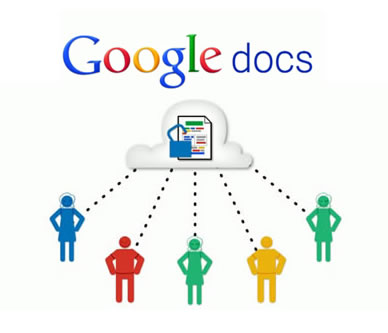
\includegraphics[scale=0.8]{figuras/googledocs.jpg}\\
  \caption{GoogleDocs}\label{fig:googledocs}
\end{figure}





\section{Técnicas y herramientas para el aprendizaje colaborativo}

\subsection{Sistema Web para la enseñanza de Casos
de Uso empleando la Técnica de Aprendizaje Cooperativo
de Rompecabezas.}

Este sistema es producto de una tesis de grado implementada en la Pontificia Universidad Católica del Perú. El sistema pretende dar soporte a las tres fases que comprende una clase en la cual se emplea la técnica de Jigsaw para lo cual, se construyeron los módulos de Planificación, Ejecución y Evaluación.\\

El módulo de Planificación permite realizar el diseño de cada sesión de clase. Ahí se plantean los datos de la sesión que serán la base de los objetivos y resultados esperados que permitirán medir el progreso académico de los alumnos.\\

El módulo de Ejecución se encarga de llevar a cabo la ejecución de una sesión de clase basada en la técnica de Jigsaw. Permite el desarrollo paso a paso desde la lectura de materiales, documentos y casos hasta la diagramación de la solución que brinden cada uno de los grupos Jigsaw y Expertos. En este módulo se cuenta con foros de discusión que permiten la comunicación entre los miembros de cada grupo.\\

Por último se tiene el módulo de Evaluación, en el cual se elaboran preguntas y examenes que luego el profesor aplica a sus alumnos. Estos exámenes son calificados manualmente o de forma automática por el propio sistema.

\subsubsection{Arquitectura del sistema}
El sistema fue desarrollado usando una arquitectura Modelo-Vista-Controlador. Se usó Java como plataforma de desarrollo y MySQL como motor de base de datos. Acontinuación se indican los frameworks utilizados en el sistema:

\begin{itemize}
  \item Framework J2EE
  \item Struts 2
  \item MyBatis
  \item Librerías AJAX: JQuery, DojoToolKit
\end{itemize}
\emph{Fuente} \cite{pinzas_desarrollo_2013}

\subsection{CodeBunks}
Es una plataforma que permite codificar y compilar en diferentes lenguajes de programación de forma colaborativa y en tiempo real.
\subsubsection{Funcionalidades}
\begin{enumerate}
  \item Posee un editor colaborativo que soporta 14 lenguajes de programación, tiene coloración de sintaxis según el lenguaje y brinda un indentado inteligente.
  \item Compilar y Ejecutar. La plataforma permite compilar y ejecutar código en Python, Java, C, C++, Ruby, Javascript, entre otros.
  \item Audio y Video Chat.
  \item Code playback. Permite repetir la historia de los cambios realizados en el código.
  \item Equipos. Permite crear equipos de trabajo e invitar a otros usuarios a colaborar en el desarrollo de un programa.
\end{enumerate}
\begin{figure}[h]
  \centering
  % Requires \usepackage{graphicx}
  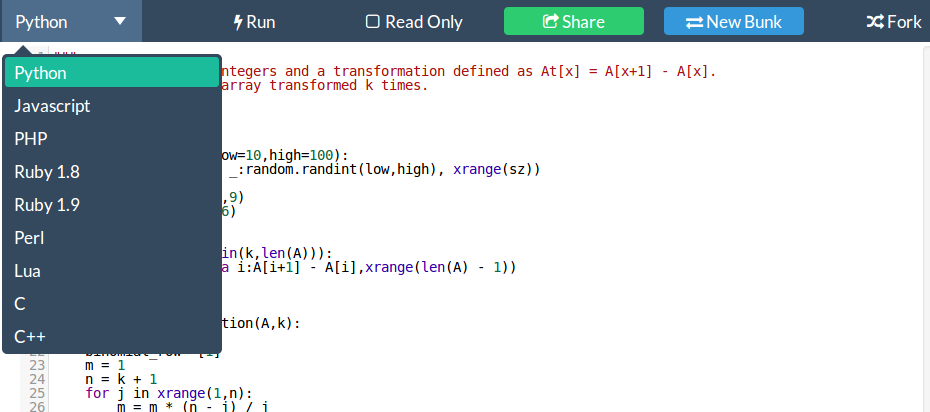
\includegraphics[scale=0.3]{figuras/codebunk.png}\\
  \caption{Codebunk}\label{fig:codebunk}
\end{figure}
\section{Frameworks para aplicaciones web de tiempo real}

\subsection{GoogleDrive Realtime API}

La API de GoogleDrive en tiempo real ofrece el trabajo colaborativo como un servicio para los archivos en Google Drive a través del uso de las transformaciones operativas. El API es una biblioteca JavaScript que ofrece a los desarrolladores objetos de colaboración, eventos y métodos para la creación de aplicaciones en las cuales se puedan realizar tareas colaborativas.\\

Esta API permite a los desarrolladores diseñar un modelo de datos común que se ve como un modelo local en memoria. Se pueden escribir código para manipular listas, arrays, matrices, maps, y objetos javascript propios del desarrollador. Cada vez que se modifique un modelo de datos, éste automáticamente cambiará para todos los usuarios presentes en el documento.\\

La API está basada en la misma tecnología de colaboración usada por GoogleDocs y por ello, cada vez que un modelo de datos es modificado, el cambio es aplicado inmediatamante a la copia local del documento y luego, la API envía una representación del cambio al servidor de tal forma que el cambio es guardado en el documento y comunicado a los demás colaboradores.\\

La API en tiempo real se encarga de todos los aspectos de la transmisión de datos, el almacenamiento y la resolución de conflictos cuando varios usuarios están editando un archivo. En general, la API nos brinda lo siguiente:

\begin{enumerate}
  \item Funciones para cargar y trabajar documentos en tiempo real.
  \item Objetos construídos colaborativamente(cadenas, listas, y mapas).
  \item La capacidad de crear objetos propios que puedan personalizarse.
  \item Eventos para la detección de cambios en el modelo de colaboración y detección del ingreso o salida de colaboradores.
\end{enumerate}
La API en tiempo real de GoogleDrive proporciona todas las herramientas que se necesitan para crear una aplicación colaborativa que no necesita correr en nuestro propio servidor.



\subsection{NodeJS}
\subsection{Socket.IO}

Socket.IO permite la comunicación basada en eventos bidireccional en tiempo real.
Funciona en todas las plataformas, el navegador o dispositivo, centrándose también en la fiabilidad y la velocidad.
\begin{itemize}
  \item Análisis en tiempo real
  \item Transmisión binaria. A partir de 1.0, es posible enviar cualquier tipo de archivo: imagen, audio, video.
  \item Mensajería instantánea y chat
  \item Colaboración de documentos. Permitir a los usuarios editar simultáneamente un documento y ver los cambios del otro.
\end{itemize}





\section{Algoritmos y programación}
\subsection{Estructura de datos}
\subsection{Búsqueda y Ordenamiento}
\subsection{Programación orientada a objetos}
